\documentclass[12pt]{article}

\setlength{\parindent}{0pt}
\setcounter{secnumdepth}{3}
\usepackage[margin=1in]{geometry}

% packages
\usepackage{amsmath, amsfonts, amsthm, amssymb}
\usepackage{graphicx, float}
\usepackage{mathtools}
\usepackage{titlesec}
\usepackage{interval}
\usepackage{hyperref}
\usepackage{siunitx}
\usepackage{titling}
\usepackage{vwcol}
\usepackage{setspace}
\usepackage{empheq}
\usepackage{cancel}
\usepackage{esdiff}
\usepackage{multicol}
\usepackage{mdframed}
\usepackage{esdiff}
\usepackage{tikzsymbols}
\usepackage{multicol}
\usepackage{tikz}
\usepackage{varwidth}
\usepackage{pgfplots}
\usepackage{fancyhdr}
\usepackage{enumitem}
\usepackage{tcolorbox}

\intervalconfig {
	soft open fences
}

% header
\pagestyle{fancy}
\fancyhf{}
\lhead{Ethan Fan}
\rhead{PCH}
\cfoot{\thepage}

% section format
\titleformat{\section}
  {\bfseries}
  {}
  {0em}
  {}
\titlespacing*{\section}{0pt}{0pt}{0.3em}

\titleformat{\subsection}[runin]
  {\bfseries}
  {}
  {0em}
  {}
\titlespacing*{\subsection}{0pt}{0pt}{0em}

\titleformat{\subsubsection}[runin]
  {\itshape}
  {(\roman{subsubsection})}
  {0em}
  {}

% commands
\newcommand{\alignedintertext}[1]{%
  \noalign{%
    \vskip\belowdisplayshortskip
    \vtop{\hsize=\linewidth#1\par
    \expandafter}%
    \expandafter\prevdepth\the\prevdepth
  }%
}

\newcommand*{\paren}[1]{\ensuremath\left(#1\right)}
\newcommand*{\limit}[2][x]{\ensuremath{\displaystyle\lim_{#1\to#2}}}
\newcommand*{\Limit}[3][x]{\ensuremath{\displaystyle\lim_{#1\to#2}\left[#3\right]}}
\newcommand*{\deriv}[1][x]{\ensuremath{\dfrac{\mathrm{d}}{\mathrm{d}#1}}}
\newcommand*{\Deriv}[2][x]{\ensuremath{\dfrac{\mathrm{d}}{\mathrm{d}#1}\left[#2\right]}}
\newcommand{\dydx}{\frac{dy}{dx}}
\newcommand*{\iinteg}[2][x]{\ensuremath{\displaystyle\int #2\;\mathrm{d}#1}}
\newcommand*{\dinteg}[4][x]{\ensuremath{\displaystyle\int_{#2}^{#3}#4\;\mathrm{d}#1}}
\newcommand*{\abs}[1]{\ensuremath{\left|#1\right|}}
\newcommand*{\eps}{\varepsilon}
\newcommand*{\real}{\ensuremath\mathbb{R}}
\newcommand*{\integer}{\ensuremath\mathbb{Z}}
\newcommand*{\posint}{\ensuremath\mathbb{Z^+}}
\newcommand*{\cbrt}[1]{\ensuremath{\sqrt[3]{#1}}}
\newcommand*{\lheqzero}{\ensuremath{\underset{\text{L'H}}{\overset{\left[\frac00\right]}{=}}}}
\newcommand*{\lheqinfty}{\ensuremath{\underset{\text{L'H}}{\overset{\left[\frac{\infty}{\infty}\right]}{=}}}}
\newcommand{\tor}{\text{ or }}
\newcommand{\floor}[1]{\lfloor #1 \rfloor}

\newcommand{\vem}{\vspace{0.5em}}
\newcommand{\example}[1]{\section{Example #1}}
\newcommand{\problem}[1]{\section{Problem #1}}
\newcommand{\subproblem}[1]{\subsection{(#1)} \,}

\DeclareMathOperator{\dne}{DNE}
\DeclareMathOperator{\sgn}{sgn}

\newcommand{\definition}[1]{\begin{tcolorbox}[colback=red!5!white,colframe=red!75!black,parbox=false] #1 \end{tcolorbox}}

\newcommand{\theorem}[2]{\begin{tcolorbox}[title={#1},colback=blue!5!white,colframe=blue!75!black,parbox=false] #2 \end{tcolorbox}}

\allowdisplaybreaks
% \postdisplaypenalty=100000

% document
\begin{document}

\vspace*{0cm}

% opening
\begin{center}
    {\Large \bfseries Problem Set 68} \\[0.5cm]
    {\large The Mean Value Theorem} \\[0.35cm]
    {\normalsize April 22, 2026}
\end{center}

% problems

\problem{1}
Verify that the function satisfies the three hypotheses of Rolle's Theorem on the given interval. Then find all numbers that satisfy the conclusion of Rolle's Theorem. \vem

\subproblem{b} $f(x)=\sqrt{x}-\dfrac{x}{3}, \quad [0,9]$
\begin{enumerate}
    \item $f(x)$ is continuous on $[0,9]$ as $f(x)$ is constructed by polynomial functions and $x\ge 0$.
    \item $f(x)$ is differentiable on $(0,9)$.
    \item $\begin{cases}
        f(0)=\sqrt{0}-\dfrac{0}{3}=0 \vem  \\
    f(9)=\sqrt{9}-\dfrac{9}{3}=0
    \end{cases} \implies f(0)=f(9)$
\end{enumerate}
By Rolle's Theorem,
\begin{gather*}
    \boxed{\exists c \in (0,9) \text{ s.t. } f'(c)=0}\\
    f'(c)=\frac{1}{2\sqrt{c}}-\frac{1}{3}=0\\
    2\sqrt{c}=3\\
    \boxed{c=\frac{9}{4}}
\end{gather*}

\problem{4}
\subproblem{a} Use Desmos to graph the function $f(x)=x+\dfrac{4}{x}$ in the viewing window $[0,10]$ by $[0,10]$.
\begin{figure}[H]
    \centering
    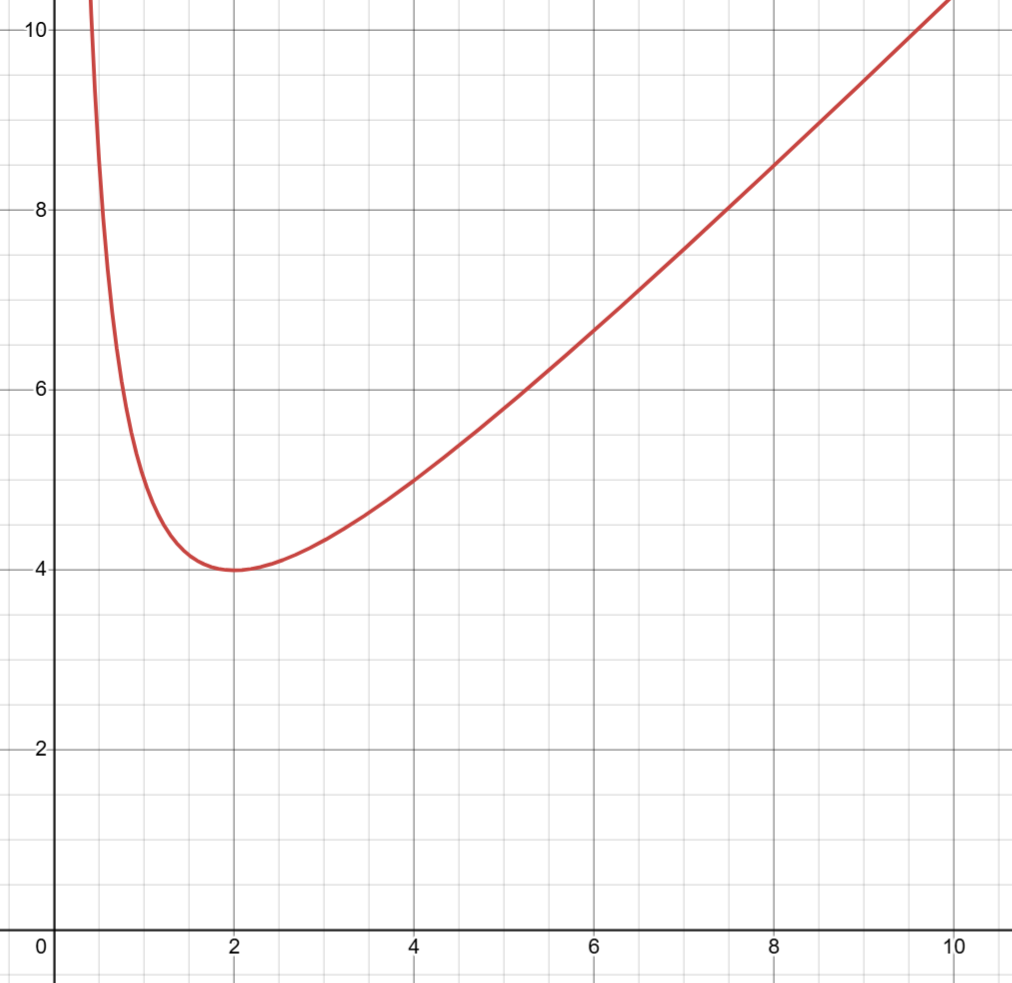
\includegraphics[width=0.4\linewidth]{q4desmos.png}
\end{figure}

\subproblem{b}
Graph the secant line that passes through the points $(1,5)$ and $(8,8.5)$ on the same screen with $f$.
\begin{figure}[H]
    \centering
    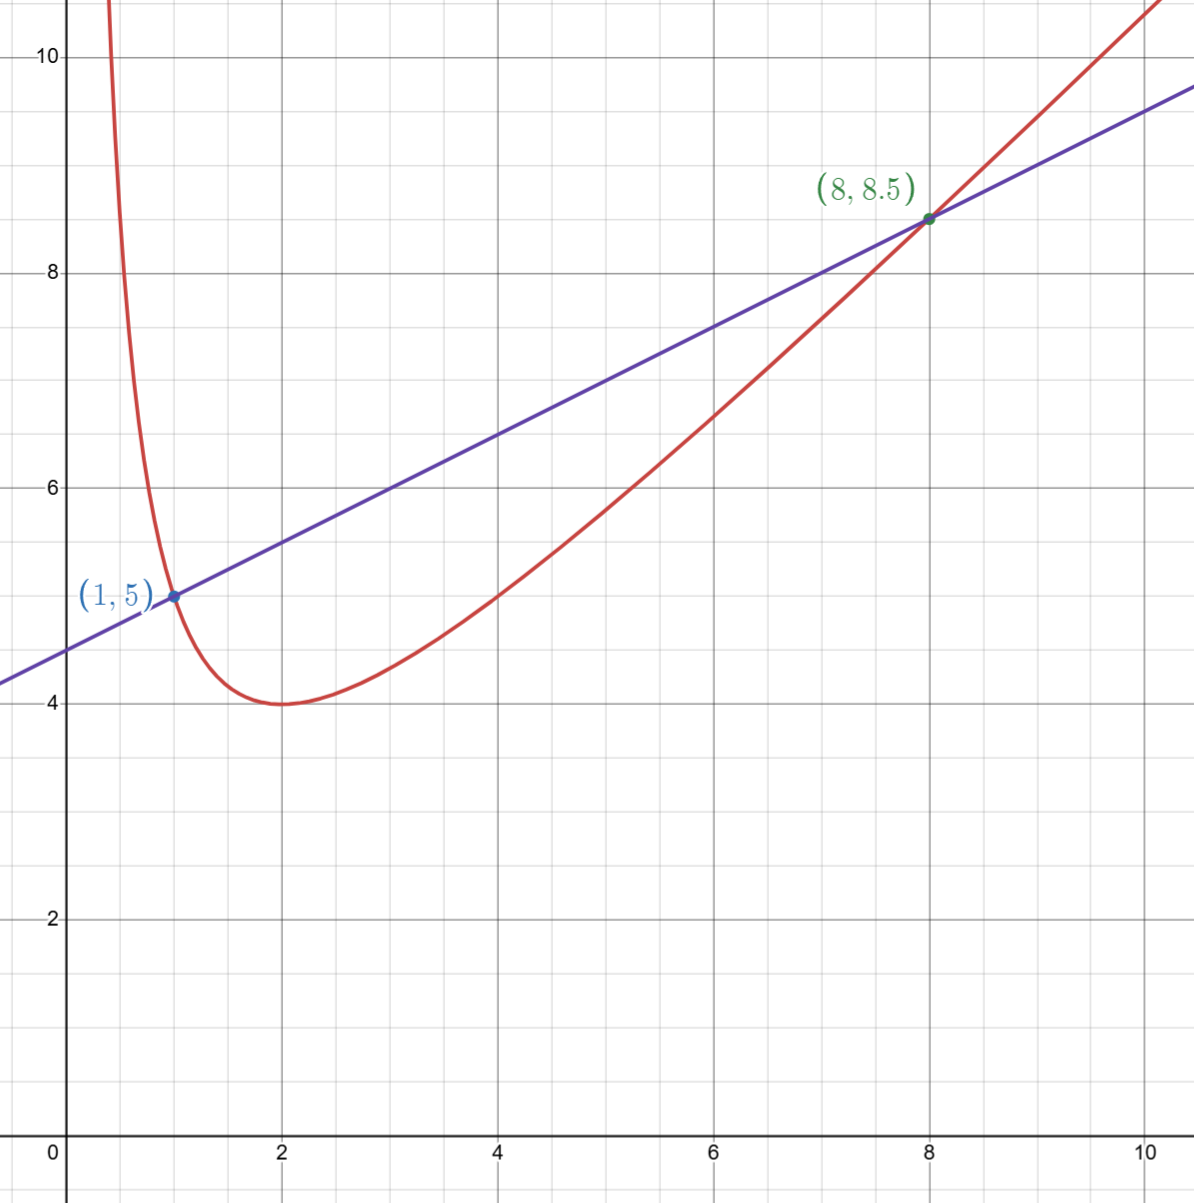
\includegraphics[width=0.4\linewidth]{q4desmos2.png}
\end{figure}

\subproblem{c}
Find the number $c$ that satisfies the conclusion of the Mean Value Theorem for this function $f$ and the interval $[1,8]$. Then graph the tangent line at the point $(c,f(c))$ and notice that it is parallel to the secant line.
\begin{gather*}
    f'(c)=1-\frac{4}{c^2}=\frac{1}{2}\\
    c^2=8\\
    \boxed{c=2\sqrt{2}}
\end{gather*}
\begin{figure}[H]
    \centering
    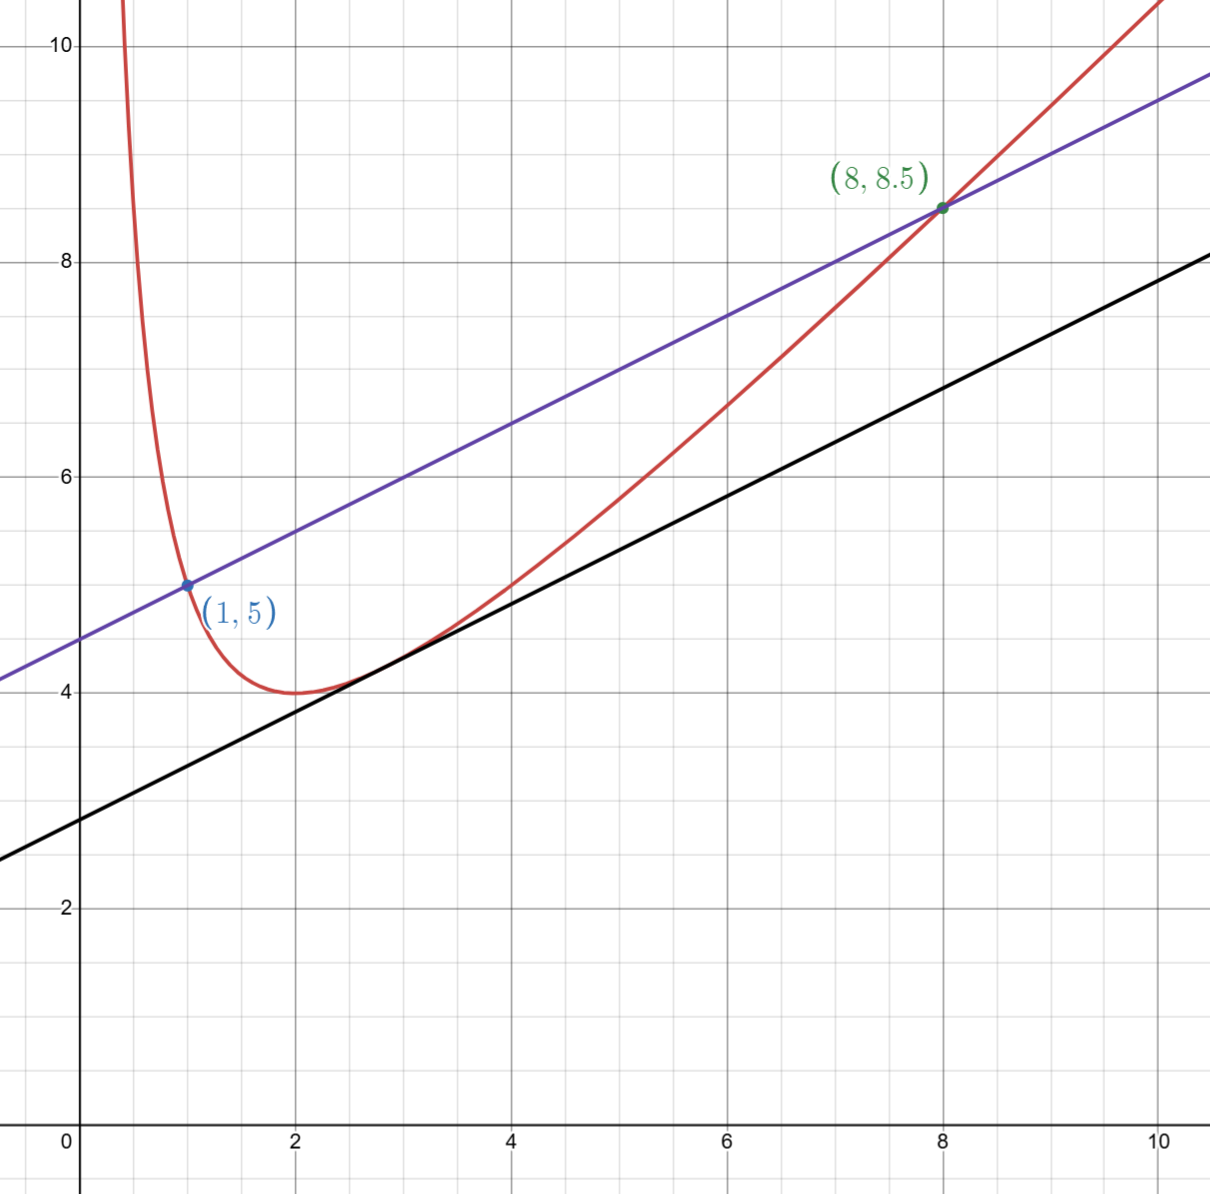
\includegraphics[width=0.4\linewidth]{q4desmos3.png}
\end{figure}

\problem{5}
Verify that the function satisfies the hypotheses of the Mean Value Theorem on the given interval. Then find all numbers $c$ that satisfy the conclusion of the Mean Value Theorem. \vem

\subproblem{a}
$f(x)=3x^2+2x+5,\quad [-1,1]$
\begin{enumerate}
    \item $f(x)$ is continuous on $[-1,1]$ as $f(x)$ is constructed by polynomial functions.
    \item $f(x)$ is differentiable on $(-1,1)$.
\end{enumerate}
By the Mean Value Theorem,
\begin{gather*}
    \boxed{\exists c \in (-1,1) $ s.t. $ f'(c)=2}\\
    f'(c)=6c+2=2\\
    \boxed{c=0}
\end{gather*}

\problem{6}
Let $f(x)=(x-3)^{-2}.$ Show that there is no value of $c$ in $(1,4)$ such that $f(4)-f(1)=f'(c)(4-1)$. Why does this not contradict the Mean Value Theorem?
\begin{gather*}
    f'(x)=-\frac{2}{(x-3)^3}\\
    f(4)=1, f(1)=\frac{1}{4}\\
    f'(c)=-\frac{2}{(c-3)^3}=\frac{1}{4}\\
    c-3=-2\\
    c=1 \implies c \notin (1,4)
\end{gather*}
As $x\ne 3$, $f(x)$ is not continuous on $[1,4]$. Hence, the conditions for the Mean Value Theorem are not satisfied. \vem 

\problem{7}
Show that the equation $1+2x+x^3+4x^5=0$ has exactly one real root. \vem \\
Given that $f(x)$ is constructed by polynomial functions, $f(x)$ is continuous and differentiable on $\mathbb{R}$.
Assume two distinct roots $a$ and $b$ satisfying $a<b$ exist. By Rolle's Theorem, there exists $c\in (a,b)$ such that $f'(c)=0$.
\begin{gather*}
    f'(x)=20x^4+3x^2+2\\
    f'(c)>0
\end{gather*}
which contradicts the assumption. Thus, $f(x)$ has exactly one real root. \vem 

\problem{9}
If $f(1)=10$ and $f'(x) \ge 2$ for $1 \le x \le 4$, how small can $f(4)$ possibly be?
\begin{gather*}
    f'(c)=\frac{f(4)-f(1)}{4-1}\\
    \frac{f(4)-10}{3}\ge 2\\
    \boxed{f(4)\ge 16}
\end{gather*}

\problem{10}
Does there exist a function $f$ such that $f(0)=-1, f(2)=4$, and $f'(x) \le 2 $ for all $x$?
\begin{gather*}
    f'(c)=\frac{f(2)-f(0)}{2-0}=\frac{5}{2}\\
    f'(c)>2\\
    \boxed{f(x)\dne}
\end{gather*}

\problem{11}
Let $f(x)=\dfrac{1}{x}$ and $g(x)=\begin{cases}
    \dfrac{1}{x} &x>0\\
    1+\dfrac{1}{x} &x<0
\end{cases}$\\
Show that $f'(x)=g'(x)$ for all $x$ in their domains. Can we conclude from the Corollary that $f-g$ is constant?
\begin{gather*}
    f'(x)=-\frac{1}{x^2}\\
    g'(x)=\begin{cases}
        -\dfrac{1}{x^2} &x>0\\
        0-\dfrac{1}{x^2} &x<0
    \end{cases}\\
    \boxed{f'(x)=g'(x), \quad  \forall x \in (-\infty ,0) \cup (0,\infty)}
\end{gather*}
No. The domain is not one single interval. \vem 

\problem{12}
Two runners start a race at the same time and finish in a tie. Prove that at some time during the race, they have the same speed. [Hint: Consider $f(t)=g(t)-h(t)$, where $g$ and $h$ are the position functions of the two runners.]
\begin{gather*}
    f(0)=g(0)-h(0)=0\\
    f(t)=g(t)-h(t)=0\\
    f(0)=f(t) \implies f'(c)=0\\
    g'(t)-h'(t)=0\\
    \boxed{g'(t)=h'(t)}
\end{gather*}

\end{document}

